\chapter{Background Contribution}\label{section:star_background}
The background contributions to the charged-particle distributions can be divided into
event-level and track-level backgrounds, and are described in detail below:
\begin{itemize}
	\item Accidental background refers to events which do not originate from a single collision of two protons.
	%\item Non-SD background comprise contibution of non-SD events which originate from a single $pp$ collision.
	\item Track backgrounds from non-primary tracks consist of secondary tracks and fake tracks; the first come mostly from decays, the short-lived particles with mean life $30 < \tau < 300$~ps, or secondary interactions with the detector dead material, while the second comes from the track reconstruction algorithms and out-of-time pile-up with
	no corresponding true particles.
\end{itemize}
%accidentals
\section{Accidental Background}\label{section:star_accidentals}
The accidental backgrounds (same bunch pile-up background) are quantified using data-driven method and defined as a process where in  single bunch crossing there is coincidence of two interactions, where any single-side proton signal is collected in coincidence with a~signal in the~TPC-TOF detector. %This has the same signature as a signal process but would not come from a DD, a CD or a ND interaction. 
This type of background may come from the overlap of a~signal in \ac{RP} (proton from beamhalo, low mass \ac{SD} process without activity in TOF, elastic or low mass \ac{CD} processes with undetected proton on the other side) with a~signal in TPC+TOF (mainly \ac{ND} events without forward proton).

The accidental background contribution was calculated  from Zerobias data, where two signatures of such background were investigated: the reconstructed proton in RP and the reconstruction of vertex from TPC tracks matched with TOF. The analysis was done for each RP arm separately and thus the 
 Zerobias data was firstly required to pass the following criteria:
\begin{enumerate}
	\item no trigger in any RP or trigger in exactly one arm (two RPs) with exactly one reconstructed proton track in that arm,
	\item veto on any signal in small BBC tiles or ZDC on the same  side of the IP as  RP under consideration,
	\item no or exactly one reconstructed vertex with at least two TOF-matched tracks passing the quality criteria. The latter includes also signal in BBC small tiles on the opposite side of the IP to the RP under study. 
\end{enumerate}
 The sample of selected Zerobias data with total  number  of events $N$ was divided into four classes:
\begin{equation}
N=N(P,S)+N(R,S)+N(P,T)+N(R,T)
\label{eq:accidentalSTAR_N}
\end{equation}
where: $N(P,S)$ is the~number of events with reconstructed proton in exactly one RP and reconstructed TOF vertex, $N(R,S)$  is the~number of events with no trigger in any RP and reconstructed TOF vertex, $N(P,T)$ is the~number of events with reconstructed proton in exactly one RP and no reconstructed TOF vertex, $N(R,T)$ is the~number of events with no trigger in any RP and no reconstructed TOF vertex.\\

Since the signature of the signal is a reconstructed proton in exactly one RP and a~reconstructed TOF vertex, the number of such events can be expressed as:
\begin{equation}
N(P,S)=N\left(p_3+p_1p_2\right)
\end{equation}
where: $p_1$ is the~probability that there is a~reconstructed proton in RP and there is no reconstructed TOF vertex, $p_2$ is the~probability that there is no reconstructed proton in RP and  there is a~reconstructed TOF vertex, $p_3$ is the~probability that there is a~reconstructed proton in RP and  there is a~reconstructed TOF vertex (not accidental).

The other classes of events given in Eq.~\eqref{eq:accidentalSTAR_N} can be expressed in terms of the~above probabilities as:
\begin{equation}
\begin{split}
N(R,S)=  & N(1-p_1)p_2(1-p_3)\\
N(P,T) = & N(1-p_2)p_1(1-p_3)\\
N(R,T) = & N(1-p_1)(1-p_2)(1-p_3)
\end{split}
\end{equation}
Finally, the accidental background contribution $A_{\mathrm{bkg} }^{\mathrm{accidental}}$ is  given by:
\begin{equation}
\begin{split}
A_{\mathrm{bkg}}^{\mathrm{accidental}}=  \frac{p_1p_2}{p_3+p_1p_2}=\frac{N(R,S)N(P,T)N}{N(R)N(T)N(P,S)}
\end{split}
\label{eq:bkg_acc_norm}
\end{equation} 
where: $N(R)=N(R,S)+N(R,T)$ and $N(T)=N(P,T)+N(R,T)$.

The shapes of the accidental background related to TPC distributions come from the~above Zerobias data events which pass all the analysis selection except having no trigger in any RP. The~templates corresponding to RP distributions are from protons in the~above data sets but with no reconstructed TOF vertex. The normalization is given by Eq.~\eqref{eq:bkg_acc_norm}. Figure~\ref{fig:STARaccidentalsXi} shows distributions of the~reconstructed $\xi$ with the~accidental background contribution  for events with proton reconstructed in EU, ED, WU and WD arms. Accidental background in the~range of $0.02<\xi<0.2$ is below $1\%$.

\begin{figure}[h!]
	\centering
	\includegraphics[width=0.49\textwidth, page=40]{chapters/chrgSTAR/img/accidentals/accidentalBkg.pdf}
	\includegraphics[width=0.49\textwidth, page=41]{chapters/chrgSTAR/img/accidentals/accidentalBkg.pdf}
	\includegraphics[width=0.49\textwidth, page=42]{chapters/chrgSTAR/img/accidentals/accidentalBkg.pdf}
	\includegraphics[width=0.49\textwidth, page=43]{chapters/chrgSTAR/img/accidentals/accidentalBkg.pdf}
	\caption{Uncorrected distributions of the reconstructed $\xi$ for events with proton reconstructed in  (top left) EU, (top right) ED, (bottom left) WU and (bottom right) WD arms. Data is shown as black markers, whereas the~accidental background contribution is shown as yellow histogram.  The ratio of accidental background and data is shown in the bottom pad.}
	\label{fig:STARaccidentalsXi}
\end{figure}

The selection of Zerobias events, which is not unique, may provide some bias to the normalization of the~accidental background. As a systematic check, two criteria for  Zerobias selection were changed~to:
 \begin{enumerate}
 	\item no trigger in any RP or trigger in exactly one arm (two RPs) with \textit{no more} than one reconstructed proton track in that arm, i.e. events with trigger signals in exactly one arm and without reconstructed proton track in that arm were also used,
 	%\item veto on any signal in small BBC tiles or ZDC on the same  side of the IP as  RP under study,
 	\item no  or exactly one reconstructed TOF vertex (%not necessarily  with two TOF-matched tracks passing the quality criteria). 
 	\textit{without any additional requirements}), i.e. events with a~reconstructed TOF vertex that does not have at least two primary tracks satisfying the~selection criteria (Sec.~\ref{section:star_track_selection}), or with a~reconstructed TOF vertex that is out of the~range of $|V_z|<80$~cm, were also accepted. The requirement of signal in BBC small tiles remains unchanged. 
 \end{enumerate}
 As a result of this change in the procedure, %, as shown in Fig.~\ref{fig:STARaccidentalsXiSyst}, 
 the accidental background normalization increases of about $50\%$ with respect to the nominal value. Therefore, the background changes by $\pm50\%$ was taken as a systematic uncertainty related to the accidentals.
 
 \begin{comment}
 \begin{figure}[h!]
 	\centering
 	\includegraphics[width=0.49\textwidth, page=40]{chapters/chrgSTAR/img/accidentals/accidentalBkg_test.pdf}
 	\includegraphics[width=0.49\textwidth, page=41]{chapters/chrgSTAR/img/accidentals/accidentalBkg_test.pdf}
 	\includegraphics[width=0.49\textwidth, page=42]{chapters/chrgSTAR/img/accidentals/accidentalBkg_test.pdf}
 	\includegraphics[width=0.49\textwidth, page=43]{chapters/chrgSTAR/img/accidentals/accidentalBkg_test.pdf}
 	\caption{Uncorrected distributions of the reconstructed $\xi$ for events with proton reconstructed in (top left) EU, (top right) ED, (bottom left) WU and (bottom right) WD arms. The~accidental background contribution calculated with changed Zerobias selection criteria is also shown.}
 	\label{fig:STARaccidentalsXiSyst}
 \end{figure}
\end{comment}




%non-SD

%background non primary
\section{Background from Non-Primary Tracks}\label{section:star_background_primary}
Reconstructed tracks matched to a~non-primary particle, so-called background tracks,  originate  mainly from the~following sources:
\begin{itemize}
	\item decays of short-lived primary particles with strange quark content (mostly $K^0$, $\Lambda^0$),
	\item photons from $\pi^0$ and $\eta$ decays which are converting to $e^+e^-$,
	\item hadronic interactions of particles with the beam-pipe or detector dead material.
\end{itemize} 

\begin{figure}[h!]
	\centering
	\begin{subfigure}{.45\textwidth}
		\includegraphics[width=\linewidth, page=1]{chapters/chrgSTAR/img/chargedBkg/bkg2D.pdf}
	\end{subfigure}
	\begin{subfigure}{.45\textwidth}
		\includegraphics[width=\linewidth, page=3]{chapters/chrgSTAR/img/chargedBkg/bkg2D.pdf}
	\end{subfigure}
\begin{comment}
	\begin{subfigure}{.45\textwidth}
		\includegraphics[width=\linewidth, page=4]{chapters/chrgSTAR/img/chargedBkg/bkg2D.pdf}
	\end{subfigure}
	\begin{subfigure}{.45\textwidth}
		\includegraphics[width=\linewidth, page=5]{chapters/chrgSTAR/img/chargedBkg/bkg2D.pdf}
	\end{subfigure}
\end{comment}
	\caption{(left) Distribution of fraction of selected tracks  associated with non-primary particles  in the~range $0.02<\xi<0.2$ and  (right) distribution of fraction of tracks which are not associated with true-level particles  in the~range $0.02<\xi<0.05$ as predicted by PYTHIA~8 4C (SaS) embedding.}
	\label{fig:bkg_fake_charged}
\end{figure}
There is also a contribution from fake tracks, i.e. tracks not associated with true-level particles, coming from out-of-time pile-up or  formed by a random combination of TPC hits. Figure~\ref{fig:bkg_fake_charged} shows the background $f_{\textrm{bkg}}\left(p_{\textrm{T}},\eta\right)$ and fake track $f_{\textrm{fake}}\left(p_{\textrm{T}},\eta\right)$ contribution to reconstructed tracks as a~function of $p_{\textrm{T}}$ and $\eta$. There were no differences observed in the~background contribution in different $\xi$ ranges, hence, all three $\xi$ ranges were merged for this study. The highest background fraction, which varies between $5-10\%$, was found to be at low $p_{\textrm{T}}$.  Due to too low statistics in PYTHIA~8 embedding \ac{MC}, the~shape of the~fake track contribution was assumed to be the~same in all three $\xi$ ranges. However, its normalization was calculated for each $\xi$ range separately with a ratio between the ranges of $1: 0.74: 1.11$.
The~change by $\pm100\%$ in fake track contribution was taken as a systematic uncertainty.


Figure~\ref{fig:bkg_epos_charged} shows the~background track contribution to reconstructed tracks as a~function of $p_\textrm{T}$ and $\eta$ calculated from EPOS SD+SD$^\prime$. The differences between
PYTHIA~8 and EPOS, which are up to $50\%$ for $p_\textrm{T}>0.5$~GeV/c (as shown in Fig.~\ref{fig:bkg_epos_charged_1D}), were symmetrized and taken as a~systematic uncertainty.




\begin{figure}[h!]
	\centering
	\begin{subfigure}{.49\textwidth}
		\includegraphics[width=\linewidth, page=7]{chapters/chrgSTAR/img/chargedBkg/bkg2D.pdf}
	\end{subfigure}
    \begin{minipage}{.49\textwidth}
    	\caption{Distribution of fraction of selected tracks  associated with non-primary particles  as predicted by EPOS SD+SD$^\prime$.}
    	\label{fig:bkg_epos_charged}
    \end{minipage}
	
\end{figure}

\begin{figure}[h!]
	\centering
	\begin{subfigure}{.45\textwidth}
		\includegraphics[width=\linewidth, page=8]{chapters/chrgSTAR/img/chargedBkg/bkg2D.pdf}
	\end{subfigure}
	\begin{subfigure}{.45\textwidth}
		\includegraphics[width=\linewidth, page=9]{chapters/chrgSTAR/img/chargedBkg/bkg2D.pdf}
	\end{subfigure}
	\caption{PYTHIA~8 SD and EPOS SD+SD$^\prime$ predictions of fraction of selected tracks  associated with non-primary particles  as a~function of (left) $p_\textrm{T}$ and (right) $\eta$.}
	\label{fig:bkg_epos_charged_1D}
	
\end{figure}

%\FloatBarrier
%background proton
\subsubsection{Proton Background}\label{section:star_background_proton}
Secondary particles can be created due to the interaction of particles with detector dead-material.
The proton sample contains background from such protons knocked out  from the~detector materials~\cite{STAR:spectra}. Most of these protons have large $\textrm{DCA}$ and are not reconstructed as primary particles. However, the rest with small $\textrm{DCA}$  are included in the primary track sample. Antiprotons do not have knockout background, hence the flat $\textrm{DCA}$ tail is almost absent from their $\textrm{DCA}$ distributions.

\begin{figure}[h!]
	\centering
	\begin{subfigure}{.49\textwidth}
		\includegraphics[width=\linewidth, page=1]{chapters/chrgSTAR/img/DCAproton/background_p_0.pdf}
	\end{subfigure}
	\begin{subfigure}{.49\textwidth}
		\includegraphics[width=\linewidth, page=2]{chapters/chrgSTAR/img/DCAproton/background_p_0.pdf}
	\end{subfigure}
	\begin{subfigure}{.49\textwidth}
		\includegraphics[width=\linewidth, page=4]{chapters/chrgSTAR/img/DCAproton/background_p_0.pdf}
	\end{subfigure}
	\begin{subfigure}{.49\textwidth}
		\includegraphics[width=\linewidth, page=5]{chapters/chrgSTAR/img/DCAproton/background_p_0.pdf}
	\end{subfigure}
	\caption{The $\textrm{DCA}$ distributions of protons for $0.4<p_T<0.5$~GeV/c shown for single range of $0.02<\xi<0.05$ (shown in log and linear scale in left and right column, respectively). The MC  constributions are shown after scaling the dead-material template  to data. (top) Background enriched samples were used in the normalization procedure, whereas (bottom) the proton background was estimated from the nominal sample.}
	\label{fig:bkg_proton}
\end{figure}

In order to correct for the knock-out background protons, sample enriched in proton background  was used for background normalization, where $\textrm{DCA}_{xy}$, $\textrm{DCA}_z$ and $d_0$ cuts were abandoned. Additionally, at least one, instead of exactly one,  reconstructed vertex was allowed in this sample.  \Cref{fig:bkg_proton,fig:bkg_proton_bar} show the~$\textrm{DCA}$ distributions of protons and antiprotons, respectively, for  nominal (bottom) and background enriched (top) samples. The distributions for other $p_\textrm{T}$ and $\xi$ regions are shown in Appendix~\ref{appendix:DCA_proton}.
The protons and antiprotons are selected by a $dE/dx$ cut of $-1 < n\sigma_{p,\bar{p}} < 3$ where $n\sigma_{p,\bar{p}}$ is given by Eq.~\eqref{eq:nsigma}. The fraction of knock-out protons within the selected sample is determined via a MC template normalization method. The templates of reconstructed tracks with $dE/dx$ corresponding to the~proton and antiproton are obtained from MC separately for:
\begin{itemize}
	\item primary (anti)protons,
	\item knock-out background protons (labeled as dead-material),
	\item fake tracks,
	\item secondary particles with $dE/dx$ of (anti)proton (labeled as wrong PID - sec.),
	\item tracks associated with primary (anti)protons, but with the reconstructed vertex  not matched to true-level primary vertex (labeled as wrong vtx),
	\item reconstructed track is partially matched to true-level particle (labeled as wrong match, track to true-level particle matching is described in~\ref{section:star_TPCeffi}), i.e.  track and true-level particle have appropriate number of common hit points but the distance between true-level particle and track is too large, $\delta^2\left(\eta,\phi\right)>\left(0.15\right)^2$, 
	\item primary particles with $dE/dx$ of (anti)proton (labeled as wrong PID - prim.),
	\item (anti)proton as a product of short-lived decays, mainly $\Lambda^0$ (labeled as feed-down).
\end{itemize}



First, the background enriched sample was used  (Fig.~\ref{fig:bkg_proton}, top), where the template of knock-out background protons was normalized to the number of events in the fake-subtracted tail of the $\textrm{DCA}$ distribution, $2<\textrm{DCA}<15$~cm. Next the knock-out proton and fake background was subtracted from the $\textrm{DCA}$ distribution and the sum of other templates was normalized to the number of events in the signal region,  $\textrm{DCA}<1.5$~cm. 

\begin{figure}[h!]
	%\vspace{-1cm}
	\centering
	\begin{subfigure}{.49\textwidth}
		\includegraphics[width=\linewidth, page=1]{chapters/chrgSTAR/img/DCAproton/background_p_bar_0.pdf}
	\end{subfigure}
	\begin{subfigure}{.49\textwidth}
		\includegraphics[width=\linewidth, page=2]{chapters/chrgSTAR/img/DCAproton/background_p_bar_0.pdf}
	\end{subfigure}
	\begin{subfigure}{.49\textwidth}
		\includegraphics[width=\linewidth, page=4]{chapters/chrgSTAR/img/DCAproton/background_p_bar_0.pdf}
	\end{subfigure}
	\begin{subfigure}{.49\textwidth}
		\includegraphics[width=\linewidth, page=5]{chapters/chrgSTAR/img/DCAproton/background_p_bar_0.pdf}
	\end{subfigure}
	\caption{The $\textrm{DCA}$ distributions of antiprotons for $0.4<p_\textrm{T}<0.5$~GeV/c shown for one range of $0.02<\xi<0.05$ (log and linear scale in left and right column, respectively). The MC controbutions are shown as colour histograms. (top) Background enriched and (bottom) nominal samples were used.}
	\label{fig:bkg_proton_bar}
	%\vspace{-1cm}
\end{figure}

The fraction of the knock-out proton background in the signal region, $\textrm{DCA}<1.5$, was estimated from the nominal sample (Fig.~\ref{fig:bkg_proton}, bottom), where $\textrm{DCA}_{xy}$, $\textrm{DCA}_z$ and $d_0$ track cuts were applied and exactly one reconstructed vertex was required. The normalization of each MC contribution was kept the same as that estimated for the background enriched sample. Figure~\ref{fig:bkg_proton_fit} shows the knock-out proton background as a function of $p_\textrm{T}$ in three ranges of $\xi$. The following functional form was found to describe the
background protons well:
\begin{equation}
f_{\textrm{bkg}}^{p}\left(p_\textrm{T}\right) = p_0\exp\left(p_1p_\textrm{T}\right)
\label{eq:protonBkgParametrization}
\end{equation}
where  $p_0$ and $p_1$ are  free parameters obtained from a~fit. 

The obtained fraction of knock-out background protons is approximately $20\%$ at $p_\textrm{T} = 0.45$ GeV/c
 and less than $10\%$ at $p_\textrm{T} = 1.0$~GeV/c. The fraction of knock-out background protons depends on a number of factors, including the amount of detector material, analysis cuts and the $\xi$ of diffractive proton. 
 
 
 
 Figure~\ref{fig:bkg_proton_bar} shows the corresponding $\textrm{DCA}$ distributions with MC templates for antiprotons, where the background form knock-out particles is not present. The MC templates  fairly well describe the $\textrm{DCA}$ distribution for both, protons and antiprotons. Additionally, there is a small $\left(<1\%\right)$ background  contribution, present for both particles, which also was taken into account and subtracted. It originates from reconstructed tracks which have the appropriate number of common hit points with true-level particle, but the distance between them is too large, i.e. $\delta^2\left(\eta,\phi\right)>\left(0.15\right)^2$.
 
 %\captionsetup{format=plain,indention=0pt,justification=justified}
 \begin{figure}[h!]% \begin{wrapfigure}{r}{0.45\textwidth}
 	\centering
 	%\vspace{-20pt}
 	\includegraphics[width=0.8\linewidth, page=1]{chapters/chrgSTAR/img/DCAproton/bkg_p.pdf}
 	%\vspace{-20pt}
 	\caption{The fraction of knock-out proton background  as a function of $p_\textrm{T}$ in three ranges of $\xi$  with  fitted parametrizations.}
 	%\vspace{-80pt}
 	\label{fig:bkg_proton_fit}
 \end{figure}
 %\captionsetup{format=default,indention=0pt,justification=justified}
 %\FloatBarrier
 
 \subsubsection{Systematic Uncertainty Related to Proton Background} 
The method of   knock-out proton background estimation  introduces independent systematic uncertainties which are added in quadrature. 

First, the normalization interval of the  knock-out   proton  background template in the background enriched sample was changed to $4<\textrm{DCA}<15$~cm. This introduced a relative systematic uncertainty of up to $30\%$ for $p_\textrm{T}\approx 1.0$~GeV/c. 

 \begin{figure}[h!]
 	\centering
 	\begin{subfigure}{.49\textwidth}
 		\includegraphics[width=\textwidth,page=1]{chapters/chrgSTAR/img/DCAproton/Ratio.pdf}
 	\end{subfigure}%\label{fig:protonBkgSystRatio}
 	\begin{subfigure}{.49\textwidth}
 		\includegraphics[width=\textwidth,page=1]{chapters/chrgSTAR/img/DCAproton/p_bkg.pdf}
 	\end{subfigure}
 	\begin{subfigure}{.49\textwidth}
 		\includegraphics[width=\textwidth,page=2]{chapters/chrgSTAR/img/DCAproton/p_bkg.pdf}
 	\end{subfigure}
 	\begin{subfigure}{.49\textwidth}
 		\includegraphics[width=\textwidth,page=3]{chapters/chrgSTAR/img/DCAproton/p_bkg.pdf}
 	\end{subfigure}
 	\caption{(top left) Data to MC ratio of  the  number of events in the background dominated region in three ranges of $\xi$ with fitted functional form given by Eq.~\eqref{eq:slopeBkgFit}. (top right and bottom) Components of the systematic uncertainty related to the  knock-out background protons contribution in three $\xi$ ranges. }
 	\label{fig:protonBkgSyst}
 	
 	%\vspace{-2.5cm}
 \end{figure}

The  knock-out proton background contribution was  parameterized as  it is shown in  Eq.~\eqref{eq:protonBkgParametrization}. The systematic uncertainty related to the fit procedure was estimated by varying the   parameters, $p_0$ and $p_1$, by their statistical uncertainties ($\pm1\sigma$).  As a result, a~relative systematic uncertainties of about $10\%$ were obtained.


 
 Figure~\ref{fig:protonBkgSyst} (top left) shows the data to MC ratio of  the  number of events in the background dominated region, $2<\textrm{DCA}<15$~cm. The shape of the $\textrm{DCA}$ distribution in data  differs from that observed in simulation. Thus, the following functional form was used to estimate the slope between data and MC:
\begin{equation}
\frac{\textrm{data}}{\textrm{MC}}\left(\textrm{DCA}\right) = A(\textrm{DCA}-8.5)+B
\label{eq:slopeBkgFit}
\end{equation}
where $A$ (slope) and  $B$ are fit free parameters. An extrapolation of the slope was used to estimate how many
more tail-like tracks would fit into the signal region and a systematic uncertainty, which varies up to $5\%$ for $0.02< \xi<0.05$, was introduced. 




All above components of the systematic uncertainty related to the knock-out proton background are shown in Fig.~\ref{fig:protonBkgSyst}.
 
 
 


 
  %\FloatBarrier
%background pion
\subsubsection{Pion Background}\label{section:star_background_pion}
The pion spectra are corrected for weak decays (mainly of $K^0_S$ and $\Lambda^0$), muon contribution and background from the   detector dead-material interactions. The pion decay muons can be identified as pions due to the similar masses. These contributions are obtained from PYTHIA~8 \ac{SD}. Figure~\ref{fig:bkg_pion} shows the background contribution to the pion spectra as a function of $p_\textrm{T}$ in three ranges of $\xi$, separately for $\pi^-$ and $\pi^+$.  Since there were   negligible differences  observed between these  three ranges of $\xi$, the background contribution was averaged over $\xi$. The following parametrization was found to describe it:
\begin{equation}
f_{\textrm{bkg}}^{\pi}\left(p_\textrm{T}\right)=a_0\exp(a_1p_\textrm{T})+a_2p_\textrm{T}^2+a_3p_\textrm{T}
\end{equation}
where $a_i$, $i=0,\dots, 3$ are free paramaters of the fitted function. 

The pion background contribution varies between $5\%$ at low-$p_\textrm{T}$  ($p_\textrm{T}=0.25$~GeV/c) and about $1\%$ at $p_\textrm{T}=1.0$~GeV/c for both negatively and positively charged pions. In addition, the~background was calculated from EPOS SD+SD$^\prime$ for the~full range of $\xi$. The~differences between PYTHIA~8 and EPOS are up to $1\%$ for $\pi^-$. 
\begin{figure}[htpb]
	\centering
	\begin{subfigure}{.49\textwidth}
		\includegraphics[width=\linewidth, page=1]{chapters/chrgSTAR/img/chargedBkg/bkg0max.pdf}
	\end{subfigure}
	\begin{subfigure}{.49\textwidth}
		\includegraphics[width=\linewidth, page=2]{chapters/chrgSTAR/img/chargedBkg/bkg0max.pdf}
	\end{subfigure}
	\caption{Pion background fraction as a function of $p_\textrm{T}$ calculated from PYTHIA~8 and shown separately for  (left) negatively  and (right)  positively charged pions in three ranges of $\xi$: (red) $0.02<\xi<0.05$,  (green) $0.05<\xi<0.1$, (blue) $0.1<\xi<0.2$.  (full black points) The pion background averaged over three ranges of $\xi$ with fitted parametrization is also shown. Open black points represent EPOS predictions for the full $\xi$ range.}
	\label{fig:bkg_pion}
\end{figure}

\FloatBarrier
